
\documentclass[a4paper,UKenglish,cleveref, autoref]{lipics-v2019}
%This is a template for producing LIPIcs articles. 
%See lipics-manual.pdf for further information.
%for A4 paper format use option "a4paper", for US-letter use option "letterpaper"
%for british hyphenation rules use option "UKenglish", for american hyphenation rules use option "USenglish"
%for section-numbered lemmas etc., use "numberwithinsect"
%for enabling cleveref support, use "cleveref"
%for enabling cleveref support, use "autoref"


\bibliographystyle{plainurl}% the mandatory bibstyle

\usepackage{graphicx}
\usepackage{algorithm}
\usepackage[noend]{algpseudocode}
\usepackage{amsmath}
\usepackage{amssymb}
%\usepackage{amsmath}
%\usepackage{amsthm}
\usepackage{mathtools}
\usepackage{latexsym}
\usepackage{amstext}
\usepackage{xspace}
\usepackage{enumerate}
\usepackage{macrosLLNCS}
\usepackage{graphicx}
\usepackage{color}
\usepackage{epstopdf}
% New definitions

\def\leaveout#1{}
\def\>{\ensuremath{\rangle}}
\def\<{\ensuremath{\langle}}
\def\h{\ensuremath{\mathcal{H}}}
\def\p{\ensuremath{\mathcal{P}}}
\def\l{\ensuremath{\mathcal{L}}}
\def\g{\ensuremath{\mathcal{G}}}
\def\lh{\ensuremath{\mathcal{L(H)}}}
\def\dh{\ensuremath{\mathcal{D(H})}}

\def\r{\ensuremath{\mathcal{R}}}

\def\ra{\ensuremath{\rightarrow}}
\def\e{\ensuremath{\mathcal{E}}}
\def\f{\ensuremath{\mathcal{F}}}

\def\c{\ensuremath{\mathcal{C}}}
\def\d{\ensuremath{\mathcal{D}}}
\def\le{\ensuremath{\sqsubseteq}}
\def\z{\ensuremath{{\bf 0}}}

\newcommand{\abis}{\stackrel{\lambda}\approx}
\newcommand{\abisa}[1]{\stackrel{#1}\approx}
\newcommand {\qbit} {\mbox{\bf{new}}}
\newcommand {\nil} {\mbox{\bf{nil}}}
\newcommand {\iif} {\mbox{\bf{if}}}
\newcommand {\then} {\mbox{\bf{then}}}
\newcommand {\eelse} {\mbox{\bf{else}}}
\newcommand {\qcf}[1] {{\sf{#1}}}
\newcommand{\con}[3]{\iif\ {#1}\ \then\ {#2}\ \eelse\ {#3}}

\newcommand{\ptr}{{\rm env}}
\newcommand{\rto}[1]{\stackrel{#1}\longrightarrow}
\newcommand{\Rto}[1]{\stackrel{#1}\Longrightarrow}
\newcommand{\nrto}[1]{\stackrel{#1}\nrightarrow}

\newcommand{\Rhto}[1]{\stackrel{\widehat{#1}}\Longrightarrow}
\newcommand{\define}{\stackrel{\it def}=}
\newcommand{\rsim}{\simeq}
\newcommand{\obis}{\approx_o}
%%%%%%%%%%%%%%%%% Distributions
\newcommand{\eDis}{\varepsilon}
\newcommand{\Stop}{{\times}}
\newcommand{\Mass}[1]{|#1|}
\newcommand{\subdist}[1]{\mathop{\mbox{$\mathcal D_{\textsl{sub}}$}}(#1)}
\newcommand{\dist}[1]{\mathop{Dist} ({#1})   } % distributions
\newcommand{\pdist}[1]{\overline{#1}  } % distributions
\newcommand{\support}[1]{\lceil{#1}\rceil}
\newcommand{\lift}[1]{\mathrel{{#1}^\circ}}

%%%%%%%%%%%%%%%% language
\newcommand{\probc}[1]{\mathrel{\!_{\scriptscriptstyle #1}\oplus}}
\newcommand{\Act}{\ensuremath{\mathsf{Act}}\xspace}

\newcommand{\setof}[2]{\{ \, #1 \, \mid \, #2 \, \}}% set comprehension
\newcommand{\Nat}{\mathbb{N}}
\newcommand{\Real}{\mathbb{R}}
\newcommand{\pair}[1]{\langle{#1}\rangle}
\newcommand{\ket}[1]{|{#1}\rangle}
\newcommand{\bra}[1]{\langle{#1}|}

%\newcommand{\so}{{\cal TSO}}
\newcommand{\Con}{{\it Con}}
\newcommand{\qv}{{\it qv}}
\newcommand{\qc}{\underline{c}}
\newcommand{\qd}{\underline{d}}
\newcommand{\cVar}{{\it cVar}}
\newcommand{\qVar}{{\it qVar}}
\newcommand{\cChan}{{\it cChan}}
\newcommand{\qChan}{{\it qChan}}
\newcommand{\tr}{{\rm tr}}
\newcommand{\CE}{{\cal E}}
\newcommand{\CH}{{\cal H}}
\newcommand{\CL}{{\cal L}}
\newcommand{\CC}{{\cal C}}
\newcommand{\CD}{{\cal D}}
\newcommand{\ifthen}[2]{{\textbf{if} ~#1~ \textbf{then} ~#2}}

\algnewcommand\algorithmicswitch{\textbf{switch}}
\algnewcommand\algorithmiccase{\textbf{case}}
\algnewcommand\algorithmicotherwise{\textbf{otherwise}}
\algnewcommand\algorithmicassert{\texttt{assert}}
\algnewcommand\Assert[1]{\State \algorithmicassert(#1)}%
% New "environments"
\algdef{SE}[SWITCH]{Switch}{EndSwitch}[1]{\algorithmicswitch\ #1\ \algorithmicdo}{\algorithmicend\ \algorithmicswitch}%
\algdef{SE}[CASE]{Case}{EndCase}[1]{\algorithmiccase\ #1}{\algorithmicend\ \algorithmiccase}%
\algdef{SE}[CASE]{Otherwise}{EndOtherwise}[1]{\algorithmicotherwise\ #1}{\algorithmicend\ \algorithmicotherwise}%
\algtext*{EndSwitch}%
\algtext*{EndCase}%
\algtext*{EndOtherwise}%
\usepackage{tabularx}
\usepackage{array}
\newcommand{\tabincell}[2]{\begin{tabular}{@{}#1@{}}#2\end{tabular}}

% New "environments"
\algdef{SE}[SWITCH]{Switch}{EndSwitch}[1]{\algorithmicswitch\ #1\ \algorithmicdo}{\algorithmicend\ \algorithmicswitch}%
\algdef{SE}[CASE]{Case}{EndCase}[1]{\algorithmiccase\ #1}{\algorithmicend\ \algorithmiccase}%
\algdef{SE}[CASE]{Otherwise}{EndOtherwise}[1]{\algorithmicotherwise\ #1}{\algorithmicend\ \algorithmicotherwise}%
\algtext*{EndSwitch}%
\algtext*{EndCase}%
\algtext*{EndOtherwise}%
\usepackage{tabularx}
\usepackage{array}
%\newcommand{\tabincell}[2]{\begin{tabular}{@{}#1@{}}#2\end{tabular}}









\title{Verifying Quantum Communication Protocols with Ground Bisimulation}
%{Checking Ground Bisimilarity for Quantum Processes}

\titlerunning{}%optional, please use if title is longer than one line

%\author{Xudong Qin}{Dummy University Computing Laboratory, [optional: Address], Country \and My second affiliation, Country \and \url{http://www.myhomepage.edu} }{johnqpublic@dummyuni.org}{https://orcid.org/0000-0002-1825-0097}{(Optional) author-specific funding acknowledgements}%TODO mandatory, please use full name; only 1 author per \author macro; first two parameters are mandatory, other parameters can be empty. Please provide at least the name of the affiliation and the country. The full address is optional
\author{Xudong Qin}{Shanghai Key Laboratory of Trustworthy Computing, East China Normal University, China}{marsxd@gmail.com}{}{}

\author{Yuxin Deng}{Shanghai Key Laboratory of Trustworthy Computing, East China Normal University, China}{yxdeng@sei.ecnu.edu.cn}{}{}

%\author{Joan R. Public\footnote{Optional footnote, e.g. to mark corresponding author}}{Department of Informatics, Dummy College, [optional: Address], Country}{joanrpublic@dummycollege.org}{[orcid]}{[funding]}

\authorrunning{X. Qin and Y. Deng}%TODO mandatory. First: Use abbreviated first/middle names. Second (only in severe cases): Use first author plus 'et al.'

\Copyright{Xudong Qin and Yuxin Deng}%TODO mandatory, please use full first names. LIPIcs license is "CC-BY";  http://creativecommons.org/licenses/by/3.0/

\ccsdesc[500]{Theory of computation~Process calculi}
\ccsdesc[300]{Theory of computation~Operational semantics}
%\ccsdesc[100]{General and reference~General literature}
%\ccsdesc[100]{General and reference}%TODO mandatory: Please choose ACM 2012 classifications from https://dl.acm.org/ccs/ccs_flat.cfm 

\keywords{Quantum process algebra, Bisimulation,
Verification, Quantum communication protocols}%TODO mandatory; please add comma-separated list of keywords

\category{}%optional, e.g. invited paper

\relatedversion{}%optional, e.g. full version hosted on arXiv, HAL, or other respository/website
%\relatedversion{A full version of the paper is available at \url{...}.}

\supplement{}%optional, e.g. related research data, source code, ... hosted on a repository like zenodo, figshare, GitHub, ...

%\funding{(Optional) general funding statement \dots}%optional, to capture a funding statement, which applies to all authors. Please enter author specific funding statements as fifth argument of the \author macro.

% \acknowledgements{I want to thank \dots}%optional

%\nolinenumbers %uncomment to disable line numbering

%\hideLIPIcs  %uncomment to remove references to LIPIcs series (logo, DOI, ...), e.g. when preparing a pre-final version to be uploaded to arXiv or another public repository

%Editor-only macros:: begin (do not touch as author)%%%%%%%%%%%%%%%%%%%%%%%%%%%%%%%%%%
\EventEditors{John Q. Open and Joan R. Access}
\EventNoEds{2}
\EventLongTitle{42nd Conference on Very Important Topics (CVIT 2016)}
\EventShortTitle{CVIT 2016}
\EventAcronym{CVIT}
\EventYear{2016}
\EventDate{December 24--27, 2016}
\EventLocation{Little Whinging, United Kingdom}
\EventLogo{}
\SeriesVolume{42}
\ArticleNo{23}
%%%%%%%%%%%%%%%%%%%%%%%%%%%%%%%%%%%%%%%%%%%%%%%%%%%%%%

\begin{document}

\maketitle

%TODO mandatory: add short abstract of the document
\begin{abstract}
	
One important application of quantum process algebras is to formally verify quantum communication protocols. With a suitable notion of behavioural equivalence and a decision method, one can determine if the specification of a protocol is consistent with an implementation. Ground bisimulation is a convenient behavioural equivalence for quantum processes because of its associated coinduction proof technique. We exploit this technique to design and implement an on-the-fly algorithm to check if two given processes in quantum CCS are equivalent, which enables us to develop a tool that can verify interesting quantum protocols such as the BB84 quantum key distribution scheme.
\end{abstract}

\section{Introduction}
\label{sec:introduction}
Process algebras provide a useful formal method for specifying and verifying concurrent systems. Their extensions to the quantum setting have also appeared in the literature. For example, Jorrand and Lalire \cite{JL04,La06} defined the \emph{Quantum Process Algebra} (QPAlg) and presented a branching bisimulation to identify quantum processes with the same branching structure. Gay and Nagarajan~\cite{GN05}  developed \emph{Communicating Quantum Processes} (CQP), for which Davidson~\cite{Da11} established a bisimulation congruence.
Feng et al. \cite{FDJY07} have proposed a quantum variant of  Milner's CCS \cite{ccs}, called qCCS, and a notion of probabilistic bisimulation for quantum processes, which is then improved to be a general notion of bisimulation that enjoys a congruence property \cite{FDY11}. Later on, motivated by~\cite{San96}, Deng and Feng~\cite{DF12} defined an open bisimulation for quantum processes that makes it possible to separate ground bisimulation and the closedness under super-operator applications, thus providing not only a neater and simpler definition, but also a new technique for proving bisimilarity.
In order to avoid the problem of instantiating quantum variables by potentially infinitely many quantum states, Feng et al. \cite{FDY14} extended the idea of symbolic bisimulation~\cite{HL95} for value-passing CCS and provided a 
 symbolic version of open bisimulation for qCCS. They also proposed an algorithm for checking symbolic ground bisimulation.
 Kubota et al. \cite{KKKKS16}  implemented a software tool to decide bisimilarity of
qCCS configurations, and used it to check the security of BB84 quantum key distribution protocol~\cite{BB84}.

In the current work, we consider the ground bisimulation proposed in \cite{DF12}. We put forward an on-the-fly algorithm to check if two given processes in qCCS with fixed initial quantum states are ground bisimilar. The algorithm is simpler than the one in \cite{FDY14} because the initial quantum states are determined for the former but can be parametric for the latter. Therefore, it is easier to implement. Moreover, in many applications, we are only interested in the correctness of a quantum protocol with a predetermined input of quantum states. This is especially the case in the design stage of a protocol or in the debugging of a program. 

The new algorithm is obtained by adapting the on-the-fly algorithm for checking probabilistic bisimulations \cite{Deng15}, which in turn has its root in similar algorithms
for checking classical bisimulations \cite{FM90,HL95}. The basic idea is as follows. A quantum process with an initial quantum state forms a configuration. We describe the operational behavour of a configuration as a probabilistic labelled transition system (pLTS), where probabilistic transitions arise naturally because measuring a quantum system can entail a probability distribution of post-measurement quantum systems. The notion of ground bisimulation is a strengthening of probabilistic bisimulation by imposing some constraints on quantum variables and the environment states of processes. Therefore, the skeleton of the algorithm for quantum ground bisimulation resembles to that for probabilistic bisimulaiton.
We have developed a tool that can check if two given configurations are ground bisimilar. It is useful to validate whether the specification of a protocol is equivalent to an implementation. We have conducted experiments on a few interesting quantum protocols including super-dense coding, teleportation, secret sharing, and the BB84 protocol.

\subparagraph*{Other related Work} 
The work closest to ours is \cite{DBLP:journals/tocl/Ardeshir-Larijani18}, where Ardeshir-Larijani et al.
have proposed a quantum variant of CCS \cite{ccs}  to describe quantum protocols. The syntax of that variant is similar to qCCS but its semantics is very different. The behaviour of a concurrent process is a finite tree and an interleaving is a path from the root to a leaf. By interpreting an interleaving as a superoperator \cite{Sel04}, the semantics of a process is a set of superoperators. The equivalence checking between two processes boils down to the equivalence checking between superoperators, which is accomplished by using the stabilizer simulation algorithm given by Aaronson and Gottesman \cite{AG04}. Ardeshir-Larijani et al. have implemented their approach in an equivalence checker in Java and verified several quantum protocols from teleportation to secret sharing. 
However, they are not able to handle the BB84 quantum key distribution protocol because its correctness cannot be specified as an equivalence between interleavings.
Our approach is based on ground bisimulation and keeps all the branching behaviour of a concurrent process. Our algorithm of checking ground bisimulations is influenced by the on-the-fly algorithm of Hennessy and Lin for value-passing CCS \cite{HL95} and inspired by the probabilistic bisimulation checking algorithm of Baier et al. \cite{BEM00}.



Besides equivalence checking, based on either superoperators or bisimulations as mentioned above, model-checking is another feasible approach to verify the correctness of quantum programs. For instance, Feng et al.~\cite{FYY13} have proposed an quantum extension of PCTL \cite{HJ94} and developed a quantum model-checking algorithm for quantum Markov Chains. The algorithm is used for model-checking the correctness of the basic BB84 protocol.

\section{Preliminaries}
\label{sec:plts}
We review the model of probabilistic labelled
transition systems (pLTSs). Later on we will interpret the behaviour
of quantum processes in terms of pLTSs because quantum measurements give rise to probability distributions naturally.

We begin with some notations. A (discrete) probability distribution
over a set $S$ is a function $\Delta : S \rightarrow [0, 1] $ with
$\sum_{s\in S} \Delta(s) = 1$; the support of such a $\Delta$ is
the set $\support{\Delta} = \setof{s \in S}{\Delta(s) > 0}$.
The point distribution $\pdist{s}$ assigns probability
$1$ to $s$ and $0$ to all other elements of $S$, so that
$\support{\pdist{s}} = \{s\}$. In this paper we only need to use distributions with finite support, and let $\dist{S}$ denote the set of
finite support distributions over $S$, ranged over by $\Delta,\Theta$ etc.
If $\sum_{k \in K} p_k = 1$ for some
collection of  $p_k \geq 0$, and the $\Delta_k$ are distributions,
then so is $\sum_{k \in K}p_k \cdot \Delta_k$ with
$(\sum_{k \in K}p_k \cdot \Delta_k)(s)~=~\sum_{k\in K} p_k\cdot \Delta_k(s).$


\begin{definition}\label{def:LTS}
	A \emph{probabilistic labelled transition system}
	is a triple
	$\langle S, \Act,  \rightarrow  \rangle$, where
	$S$ is a set of states,
	$\Act$ is a set of actions, and $\rightarrow \subseteq
	S \times \Act \times \dist{S}$ is the transition relation.
\end{definition}

We often write $s\ar{\alpha}\Delta$ for $(s,\alpha,\Delta)\in\rightarrow$, and $s\ar{\alpha}$ for $\exists \Delta: s\ar{\alpha}\Delta$.
In a pLTS actions are only performed by states, in that actions are
given by relations from states to distributions. But in general we
allow distributions over states to perform an action. For this
purpose, we \emph{lift} these relations so that they also apply to
distributions \cite{DGHM09}.
\begin{definition}\label{def:lift}
	Let  $\mathord{\aRel} \subseteq
	S\times\dist{S}$ be a relation from states to distributions in a pLTS.
	Then $\mathord{\lift{\aRel}} \subseteq \dist{S} \times
	\dist{S}$ is the smallest relation that satisfies the two rules:
	(i) $s \aRel \Theta$ implies $\pdist{s} \lift{\aRel} \Theta$;
	(ii) $\Delta_i \lift{\aRel} \Theta_i$ for all $i\in I$ implies
	$(\sum_{i\in I}p_i\cdot\Delta_i)\lift{\aRel}(\sum_{i\in I}p_i\cdot\Theta_i)$
	for any $p_i \in [0,1]$ with $\sum_{i\in I}p_i = 1$, where $I$ is a
	countable index set.
\end{definition}
\noindent

We apply this operation to the relations  $\ar{\alpha}$ in the pLTS
for $\alpha\in \Act_{\tau}$, where we also write $\ar{\alpha}$ for
$\lift{(\ar{\alpha})}$. Thus as source of
a relation $\ar{\alpha}$ we now also allow distributions.
But note that  $\pdist{s} \ar{\alpha} \Delta$ is more general than
$s \ar{\alpha} \Delta$ because if
$\pdist{s}\ar{\alpha}\Delta$ then there is a collection of distributions
$\Delta_i$ and probabilities $p_i$ such that $s\ar{\alpha}\Delta_i$ for each $i\in I$ and
$\Delta=\sum_{i\in I}p_i\cdot\Delta_i$ with $\sum_{i\in I}p_i=1$.

Let $\aRel\ \subseteq S \times S$ be a relation between states. It induces a special relation $\hat{\aRel}\subseteq S\times\dist{S}$ between states and distributions by letting
$\hat{\aRel} \define \sset{(s,\pdist{t})\mid s\aRel t}.$
Then we can use Definition~\ref{def:lift} to lift $\hat{\aRel}$ to be a relation $\lift{(\hat{\aRel})}$ between distributions. For simplicity, we combine the above two lifting operations and directly write $\lift{\aRel}$ for $\lift{(\hat{\aRel})}$ in the sequel, with the intention that a relation between states can be lifted to a relation between distributions via a special application of Definition~\ref{def:lift}. In this particular case, it holds that $\Delta \lift{\aRel} \Theta$ implies $\Theta \lift{(\aRel^{-1})}\Delta$, where $s \aRel t$ iff $t\aRel^{-1} s$ for any $s,t\in S$. This way of lifting relations has elegant mathematical characterisations; see \cite{Deng15} %{DD11} 
for more details.
\begin{proposition}

\end{proposition}


\section{Quantum CCS}\label{sec:qccs}

We introduce a quantum extension of classical CCS (qCCS) which was originally studied in \cite{FDJY07,YFDJ09,FDY11}. Three types of data are considered in qCCS: as classical data we have \texttt{Bool} for booleans and \texttt{Real} for real numbers, and as quantum data we have \texttt{Qbt} for qubits. Consequently,
two countably infinite sets of variables are assumed: $\cVar$ for classical variables, ranged over by $x,y,...$, and $\qVar$ for quantum variables, ranged over by $q,r,...$.
We assume a set ${\it Exp}$, which includes $\cVar$ as a subset and is ranged over by $e,e',\dots$,  of classical data expressions over
\texttt{Real}, and a set of boolean-valued expressions ${\it BExp}$, ranged over by $b, b',\dots$, with the usual  boolean constants $\texttt{true}$, $\texttt{false}$, and operators
$\neg$, $\wedge$, $\vee$, and $\ra$. In particular, we let $e\bowtie e'$ be a boolean expression for any $e,e'\in {\it Exp}$ and ${\bowtie} \in\sset{>, <, \geq, \leq, =}$.
We further assume that only classical variables can occur freely in both data expressions and boolean expressions.
Two types of channels are used: $\cChan$ for classical channels, ranged over by $c,d,...$, and $\qChan$ for quantum channels, ranged over by $\qc,\qd$,.... A relabelling function $f$ is a map on $\cChan\; \cup\; \qChan$ such that $f(\cChan)\subseteq \cChan$ and $f(\qChan)\subseteq \qChan$.
Sometimes we abbreviate a sequence of distinct variables $q_1,...,q_n$ into $\tilde{q}$.

The terms in qCCS are given by:
\[\begin{array}{rcl}
P,Q &::=& \Cnil \BNFsep \tau.P \BNFsep c?x.P \BNFsep c!e.P
\BNFsep \qc?q.P \BNFsep
\qc!q.P \BNFsep \CE[\tilde{q}].P
\BNFsep M[\tilde{q};x].P \BNFsep \\
& & P + Q \BNFsep  P \Cpar Q\;
\BNFsep P[f] \BNFsep P\backslash L \BNFsep \ifthen{b}{P} \BNFsep
A(\tilde{q};\tilde{x})
\end{array}\]
where $f$ is a relabelling function and $L\subseteq \cChan\cup \qChan$ is a set of channels.
Most of the constructors are standard as in CCS \cite{ccs}.
We briefly explain a few new constructors. The process $\qc?q.P$ receives a quantum datum along quantum channel $\qc$ and evolves into $P$, while $\qc!q.P$ sends out a quantum datum along quantum channel $\qc$ before evolving into $P$. The symbol $\CE$ represents a trace-preserving super-operator applied on the systems $\tilde{q}$. The process $M[\widetilde{q};x].P$ measures the state of qubits $\widetilde{q}$
according to the observable $M$ and stores the measurement outcome into the
classical variable $x$ of $P$.

Free classical variables can be defined in the usual way, except for the fact that the variable $x$ in the quantum measurement $M[\tilde{q};x]$ is bound. A process $P$ is closed if it contains no free classical variable, i.e. $fv(P)=\emptyset$.

The set of free quantum variables for process $P$, denoted by $qv(P)$ can be inductively defined as in Figure~\ref{fig:fqv}.
\begin{figure*}[t]
	\[\small\begin{array}{rclrcl}
	qv(\Cnil) & = & \emptyset & qv(\tau.P) & = & qv(P)\\
	qv(c?x.P) & = & qv(P) & qv(c!e.P) & = & qv(P) \\
	qv(\qc?q.P) & = & qv(P)-\sset{q} & qv(\qc!q.P) & = & qv(P)\cup\sset{q} \\
	qv(\CE[\tilde{q}].P) & = & qv(P)\cup \tilde{q} &
	qv(M[\tilde{q};x].P) & = & qv(P) \cup \tilde{q}\\
	qv(P+Q) & = & qv(P)\cup qv(Q) \qquad &
	qv(P \Cpar Q) & = & qv(P)\cup qv(Q)\\
	qv(P[f]) & = & qv(P) &
	qv(P\backslash L) & = & qv(P)\\
	qv(\ifthen{b}{P}) & = & qv(P) &
	qv(A(\tilde{q};\tilde{x})) & = & \tilde{q}.
	\end{array}\]
	\caption{Free quantum variables}\label{fig:fqv}
\end{figure*}
For a process to be legal, we require that
\begin{enumerate}
	\item $q\not\in qv(P)$ in the process $\qc!q.P$;
	\item $qv(P)\cap qv(Q)=\emptyset$ in the process $P \Cpar Q$;
	\item Each constant $A(\tilde{q};\tilde{x})$ has a defining equation $A(\tilde{q};\tilde{x}) \Defs P$, where $P$ is a term with $qv(P)\subseteq\tilde{q}$ and $fv(P)\subseteq \tilde{x}$.
\end{enumerate}
The first condition says that a quantum system will not be referenced after it has been sent out. This is a requirement of the quantum no-cloning theorem. The second condition says that parallel composition $\Cpar$ models separate parties that never reference a quantum system simultaneously. 

\begin{figure*}[h]
	\[\small\begin{array}{ll}
	\slinfer[\Rlts{Tau}]{\pair{\tau.P, \rho} \ar{\tau} \pair{P, \rho}}
	&\linfer[\Rlts{C-Inp}]{v\in\texttt{Real}}{\pair{c?x.P,\rho} \ar{c?v} \pair{P[v/x],\rho}}
	\\[3pt]
	\linfer[\Rlts{C-Outp}]{v=\Op{e}}{\pair{c!e.P,\rho} \ar{c!v} \pair{P,\rho} }
	
	&
	\linfer[\Rlts{C-Com}]{\pair{P_1,\rho}\ar{c?v}\pair{P'_1,\rho}\qquad
		\pair{P_2,\rho}\ar{c!v}\pair{P'_2,\rho}
	}
	{\pair{P_1\Cpar P_2,\rho} \ar{\tau} \pair{P'_1\Cpar P'_2,\rho} }
	\\[3pt]
	\linfer[\Rlts{Q-inp}]{r\not\in qv(\qc?q.P)}
	{\pair{\qc?q.P,\rho} \ar{\qc?r} \pair{P[r/q],\rho}}
	&
	\slinfer[\Rlts{Q-Outp}]{\pair{\qc!q.P,\rho} \ar{\qc!q} \pair{P,\rho} }
	\\[3pt]
	\linfer[\Rlts{Q-Com}]{\pair{P_1,\rho} \ar{\qc?r} \pair{P'_1,\rho} \qquad \pair{P_2,\rho}\ar{\qc!r} \pair{P'_2,\rho}}
	{\pair{P_1\Cpar P_2, \rho } \ar{\tau} \pair{P'_1\Cpar P'_2, \rho}}
	&
	\slinfer[\Rlts{Oper}]{\pair{\CE[\tilde{q}].P,\rho} \ar{\tau} \pair{P,\CE_{\tilde{q}}(\rho)}}
	\\[3pt]
	\linfer[\Rlts{Meas}]{M=\sum_{i\in I}\lambda_i E^i \qquad p_i=tr(E^i_{\tilde{q}}\rho)}
	{\pair{M[\tilde{q};x].P,\rho} \ar{\tau} \sum_{i\in I}p_i \pair{P[\lambda_i/x], E^i_{\tilde{q}}\rho E^i_{\tilde{q}} / p_i}}
	&
	\\
	\linfer[\Rlts{Int}]{\pair{P_1,\rho} \ar{\alpha} \Delta\qquad qbv(\alpha)\cap qv(P_2)=\emptyset}{\pair{P_1 \Cpar P_2,\rho} \ar{\alpha} \Delta\Cpar P_2}
	%\\[3pt]
	%\linfer[\Rlts{Inp-Int}]{\pair{P_1,\rho} \ar{\qc?r} \pair{P'_1,\rho}\qquad r\not\in qv(P_2)}{\pair{P_1\Cpar P_2,\rho} \ar{\qc?r} \pair{P'_1\Cpar P_2,\rho}}
	&
	\linfer[\Rlts{Sum}]{\pair{P_1,\rho} \ar{\alpha} \Delta}{\pair{P_1+P_2,\rho} \ar{\alpha} \Delta}
	\\[3pt]
	\linfer[\Rlts{Rel}]{\pair{P,\rho} \ar{\alpha} \Delta}{\pair{P[f],\rho} \ar{f(\alpha)} \Delta[f]}
	&
	\linfer[\Rlts{Res}]{\pair{P,\rho} \ar{\alpha} \Delta \qquad cn(\alpha)\cap L=\emptyset}{\pair{P\backslash L,\rho} \ar{\alpha} \Delta\backslash L}
	\\[3pt]
	\linfer[\Rlts{Cho}]{\pair{P,\rho} \ar{\alpha} \Delta \qquad \Op{b}=\texttt{true}}{\pair{\ifthen{b}{P},\rho} \ar{\alpha} \Delta}
	&
	\linfer[\Rlts{Cons}]{\pair{P[\widetilde{v}/\widetilde{x},\tilde{r}/\tilde{q}],\rho} \ar{\alpha} \Delta \qquad A(\widetilde{x}, \tilde{q})\Defs P}{\pair{A(\widetilde{v},\tilde{r}),\rho} \ar{\alpha} \Delta}
	\end{array}\]
	\caption{Operational semantics of qCCS. Here in rule $\Rlts{C-Outp}$, $\Op{e}$ is the evaluation of $e$, and in rule $\Rlts{Meas}$, $E^i_{\tilde{q}}$ denotes the operator $E^i$ acting on the quantum systems $\tilde{q}$.\label{fig:opsem}
	}
\end{figure*}

Throughout the paper we implicitly assume the convention that processes are identified up to $\alpha$-conversion, bound variables differ from each other and they are different from free variables.

We now give the %turn to the %operational 
semantics of qCCS. For each quantum variable $q$ we assume a 2-dimensional Hilbert space $\CH_q$. For any nonempty subset $S\subseteq \qVar$ we write $\CH_S$ for the tensor product space $\bigotimes_{q\in S}\CH_q$ and $\CH_{\overline{S}}$ for $\bigotimes_{q\not\in S}\CH_q$. In particular, $\CH=\CH_{\qVar}$ is the state space of the whole environment consisting of all the quantum variables, which is a countably infinite dimensional Hilbert space.


Let $P$ be a closed quantum process and $\rho$ a density operator on $\CH$,\footnote{As $\CH$ is infinite dimensional, $\rho$ should be understood as a density operator on some finite dimensional subspace of $\CH$ which contains $\h_{\qv(P)}$.} the pair $\pair{P,\rho}$ is called a \emph{configuration}. We write $\Con$ for the set of all configurations, ranged over by $\CC$ and $\CD$.
We interpret qCCS with a pLTS whose states are all the configurations definable in the language,
and whose transitions are determined by the rules in Figure~\ref{fig:opsem}; we have omitted the obvious
symmetric counterparts to the rules \Rlts{C-Com}, \Rlts{Q-Com}, \Rlts{Int} and
\Rlts{Sum}.
The set of actions $\Act$ takes the following form, consisting of classical/quantum input/output actions.
\begin{eqnarray*}
	\sset{c?v, c!v \mid c\in \cChan, v\in\texttt{Real}}&\cup&
	\sset{\qc?r,\qc!r \mid \qc\in \qChan,r\in \qVar}
\end{eqnarray*}
%The symbol $\tau$ denotes invisible actions. We write $\Act$ for $\Act\cup\sset{\tau}$, which is ranged over by $\alpha$.
We use $cn(\alpha)$ for the set of channel names in action $\alpha$. For example, we have $cn(\qc?x)=\sset{\qc}$ and $cn(\tau)=\emptyset$.

In the first eight rules in Figure~\ref{fig:opsem}, the targets of arrows are point distributions, and we use the slightly abbreviated form $\CC\ar{\alpha}\CC'$ to mean $\CC\ar{\alpha}\pdist{\CC'}$.

The rules use the obvious extension of the function~$\Cpar$ on terms to configurations and distributions. To be precise,
$\CC\Cpar P$ is the configuration $\<Q\Cpar P,\rho \>$ where $\CC=\<Q,\rho\>$, and
$\Delta\Cpar P$ is the distribution defined by:
%\vskip -2mm
\[(\Delta\Cpar P)(\pair{Q,\rho}) \define \left\{\begin{array}{ll}
\Delta(\pair{Q',\rho}) & \mbox{if $Q=Q'\Cpar P$ for some } Q'\\
0 & \mbox{otherwise.}
\end{array}\right.\]
Similar extension applies to $\Delta[f]$ and $\Delta\backslash L$.

\begin{definition}[\cite{DF12}]
	A relation $\aRel\ \subseteq \Con\times\Con$ is a \emph{ground simulation} if
	$\CC\aRel \CD$ implies that $\qv(\CC)=\qv(\CD)$, $\ptr(\CC)=\ptr(\CD)$,
	and
	\begin{itemize}
		\item whenever $\CC\ar{\alpha} \Delta$, there is some distribution $\Theta$ with $\CD\dar{\hat{\alpha}}\Theta$ and $\Delta \lift{\aRel} \Theta$.
	\end{itemize}
	A relation $\aRel$ is a \emph{ground bisimulation} if both $\aRel$ and
	$\aRel^{-1}$ are ground simulations. Two configurations are \emph{ground bisimilar} if they are related by some ground bisimulation.
\end{definition}

\section{Algorithm}
\label{sec:algorithm}
In this section, we present an on-the-fly algorithm to check if two configurations are ground bisimilar.
For convenience, we will only consider pLTSs with finite tree structures. On the one hand, this makes the algorithm easier to describe and analyse. On the other hand, our main motivation of this work is to verify quantum communication protocols and, to the best of our knowledge, almost all of them can be specified by qCCS processes without recursion.
Modifying the algorithm to deal with pLTSs with loops is possible, with an increased (but still polynomial) time complexity.

\begin{algorithm}[htbp]
\caption{Bisim(t,u)}
\label{alg:bisim}
\begin{algorithmic}[1]
\Require A pair of initial states for matching $t$,$u$.
\Ensure A boolean value $\theta$ showing if two pLTSs are bisimilar, a set of non-bisimilar state pairs $N$ and a set of bisimilar state pairs $B$.
\Function{\textbf{Bisim}}{$t,u$}
\State \textbf{return} \textbf{Match}(\textit{t,u,W})
\EndFunction
\State
\Function{\textbf{Match}}{$t,u,W$}\Comment{$t=\langle P,\rho\rangle\ and\ u=\langle Q,\sigma\rangle$}
\If{$t,u\in W$}
    \State $\theta:=\texttt{tt}$
\Else
    \For{$\gamma\in \texttt{Act}(t,u)$}
        \State ($\theta_{\gamma} ,N_{\gamma},B_{\gamma}$):=\textbf{MatchAction}(\textit{$\gamma$,t,u,W})
    \EndFor
    \State $\theta$:=$\bigwedge_\gamma\theta_\gamma\wedge qv(P)=qv(Q)\wedge tr_{\overline{qv(P)}}(\rho)=tr_{\overline{qv(P)}}(\sigma)$
    \State $N=\bigcup_{\gamma}N_\gamma$
    \State $B=\bigcup_{\gamma}B_\gamma$
    \If{$\theta=\texttt{ff}$} $N$:=$N\cup \{(t,u)\}$ 
    \ElsIf{$\theta=\texttt{tt}$} $B$:=$B\cup \{(t,u)\}$
    \EndIf
\EndIf
\State \textbf{return} ($\theta,N,B$) 
\EndFunction
\State
\Function{\textbf{MatchAction}}{$\gamma,t,u,W$}
\Switch{$\gamma$}
\Case{$c!$}
\For{$t\xrightarrow{c!e_i}t_i$} 
 \For {$u\xrightarrow{c!e'_j}u_j$}
    \State $(\theta_{ij},N_{ij},B_{ij}):=\textbf{Match}(t_i,u_j,W\cup \{(t,u)\}$
\EndFor
\EndFor
\State \textbf{return} $(\bigwedge_{i}(\bigvee_j(\theta_{ij}\wedge e_i=e'_j))\wedge\bigwedge_{j}(\bigvee_i(\theta_{ij}\wedge e_i=e'_j)),\bigcup_{ij}N_{ij},\bigcup_{ij}B_{ij})$
\EndCase
\Case{$\tau$}
\For{$t\xrightarrow{\tau}\Delta_i$} \For{$u\xrightarrow{\tau}\Theta_j$}
    \State $(\theta_{ij},N_{ij},B_{ij}):=\textbf{MatchDistribution}(\Delta_i,\Theta_j,W\cup \{(t,u)\}$
\EndFor
\EndFor
\State \textbf{return} $(\bigwedge_{i}(\bigvee_j\theta_{ij})\wedge\bigwedge_{j}(\bigvee_i\theta_{ij}),\bigcup_{ij}N_{ij},\bigcup_{ij}B_{ij})$
\EndCase
\Otherwise{}
\For{$t\xrightarrow{\gamma}t_i$} 
\For{$u\xrightarrow{\gamma}u_j$}
    \State $(\theta_{ij},N_{ij},B_{ij}):=\textbf{Match}(t_i,u_j,W\cup \{(t,u)\}$
\EndFor
\EndFor
\State \textbf{return} $(\bigwedge_{i}(\bigvee_j\theta_{ij})\wedge\bigwedge_{j}(\bigvee_i\theta_{ij}),\bigcup_{ij}N_{ij},\bigcup_{ij}B_{ij})$
\EndOtherwise
\EndSwitch
\EndFunction
\State
\Function{\textbf{MatchDistribution}}{$\Delta,\Theta,W$}
\For{$t_i\in \lceil\Delta\rceil\text{ and }u_j\in \lceil\Theta\rceil$}
    \State $(\theta_{ij},N_{ij},B_{ij}):=\textbf{Match}(t_i,u_j,W)$
\EndFor
\State $\textit{R}$:=$\{(t_i,u_j)|(t_i,u_j)\notin \bigcup_{ij}N_{ij}\}^*$
\State \textbf{return} ($\textbf{Check}(\textit{$\Delta$,$\Theta$,$R$})\wedge\bigvee_{ij}\theta_{ij},\bigcup_{ij}N_{ij},\bigcup_{ij}B_{ij}$)
\EndFunction
% \State
% \Function{\textbf{Check}}{$\Delta,\Theta,\textit{R}$}
% \EndFunction
\end{algorithmic}
\end{algorithm}

In Algorithm~\ref{alg:bisim}, the main function is \textbf{Bisim}$(t,u)$. It initializes the start state pair $(t,u)$, the set $W$ for visited state pairs,  which is empty initially, and then searches for a bisimulation based on that initialization. 
%The difference between it and that in the previous work in several aspects.
The algorithm keeps updating two sets: the above mentioned $W$  and the set $N$ for non-bisimilar state pairs. The function \textbf{Match}$(t,u,W)$ invokes a depth-first traversal to match a pair of 
states $(t,u)$ with all their possible behaviors. There are three possibilities that two states are deemed be non-bisimilar:  (1) one state has a transition that the other cannot match, (2) they do have have the same set of free quantum variables, or (3) the density operators corresponding to their quantum registers are different. If one of the three cases takes places, we add the state pair into $N$. 

An auxiliary function \textbf{Act}$(t,u)$ is called in \textbf{Match} to discover the next action that both $t$ and $u$ can perform. If the two states have no more action to do then the function returns an empty set. If only one of them has no more action to do then the two states are immediately declared to be non-bisimilar. 
%It makes the algorithm more efficient as it terminates at an early time point if those pLTSs are indeed not bisimilar. Next we prove why we can ensure that.

The other set $W$ is updated in function \textbf{MatchAction}$(\gamma,t,u,W)$. This function discovers next pairs or states or distributions, depending on the type of transitions,  and recursively invokes the function \textbf{Match} or \textbf{MatchDistribution}. The current state pair is added to $W$ when the new functions are invoked.



The function \textbf{MatchDistribution}$(\Delta,\Theta,\textit{R})$ is called if we need to compare a pair of state distributions instead of a single pair of states. It returns a boolean value indicating whether the distributions are equivalent. In order to do so, it compares each pair of states from the supports of the two distributions. After checking the bisimilarity of these state pairs, the function generates an equivalence relation of the state pairs not contained in the set $N$ for non-bisimilar state pairs. Another auxiliary function \textbf{Check}$(\Delta,\Theta,\textit{R})$ is used to check whether $\Delta$ and $\Theta$ are related by the lifted relation $\lift{R}$. Technically, we take advantage of a nice property of the lifting operation: $\Delta\lift{R}\Theta$ if and only if the maximum flow in an appropriately constructed network is $1$ \cite{BEM00, Deng15}. There are standard algorithms for computing the maximum flow in a network; see e.g. \cite{CHM90}.
Besides the lifting condition, we check the disjunction of the returning boolean values from function \textbf{Match}. 


\leaveout{ %227
\begin{definition}[Lifting Condition]
Let $\textit{R}\subseteq Dist(Con)\times Dist(Con)$ be the (strong) open bisimulation relation between two distributions, then for any $\mu,\nu\in Dist(Con),\ \mu\textit{R}\nu$ can imply that:
\begin{item}
\item[(1)] The relation satisfies the lifting condition, that is $\mu=\sum_{i\in I}p_i\textit{C}_i$, for each $i\in I,\ \textit{C}_i\textit{R}\textit{D}_i$ for some $\textit{D}_i$, and $\nu=\sum_{i\in I}p_i\textit{D}_i$.
\item[(2)] The set $I$ is not an empty set, s.t. $\exists C,D\in Con, \mu(C)>0\wedge\nu(D)>0$.
\end{item}
\end{definition}
} %end of leaveout 227

Now let us prove the termination and correctness of the algorithm. 


\begin{theorem}[Termination]

Given two states $t$ and $u$ from two loop-free pLTSs, \textbf{Bisim(t,u)} always terminates.
\end{theorem} 
\begin{proof}
%So far there is no while-loop in the qCCS, that brings convenience to the proof of termination. 
In the absence of loops in the pLTSs, the termination of the algorithm is easy to see.
Starting from the initial pair of states, the next action to perform will be detected in function \textbf{Match}. Then it invokes function \textbf{MatchAction} to find the next new pair of states and recursively call function \textbf{Match} to check them. Each time function \textbf{MatchAction} calls function \textbf{Match} it adds the current state pair into $W$ at the same time. If we reach the leaf nodes, there is no more action, we only compare the quantum variables used and the state of quantum registers. After that, the function terminates, so do the calls to the other functions. Moreover, if there still exists actions enabled in one pLTS but not in the other, then the two pLTSs are not bisimilar and then the whole algorithm terminates. 
\end{proof}


\begin{theorem}[Correctness]\label{thm:correctness}
Given two states $t$ and $u$ from two pLTSs, \textbf{Bisim}$(t,u)$ returns \textit{true} if and only if they are ground bisimilar.
\end{theorem} 
\begin{proof}
The proof of the correctness is similar to that in~\cite{HL95}. Since our algorithm is not symbolic, our treatement of boolean constraints is easier. On the other hand, we need to deal with probability distributions and have an extra procedure \textbf{MatchDistribution} to check if two distributions are related by a lifted relation. The detailed proof is provided in Appendix~\ref{sec:correctness}. 
\end{proof}

At the end of this section, we analyse the time complexity of the algorithm.

\begin{theorem}[Complexity]
Let the number of nodes reachable from $t$ and $u$ is n. The time complexity of function \textbf{Bisim}$(t,u)$ is $O(n^5/log\ n)$. % and the space complexity of it is $O(n^2)$.
\end{theorem}
\begin{proof}
 The number of state pairs is at most $n^2$. When a state pair $(t,u)$ is examined, each transition of $t$ is compared with all transitions of $u$ with the same action. Since the pLTSs are assumed to be finite trees, the number of comparisons of transitions does not exceed some constant, say $k$. Each comparison may call the function \textbf{Check} at most once, which requires time $O(n^3/log\ n)$ if we use the maximum network flow algorithm in \cite{CHM90}. As a result, the execution time of \textbf{Bisim}$(t,u)$ is in $O(n^5/log\ n)$.
\end{proof}

\section{Experimental Results}
\label{sec:experiment}
In this section, we report an implementation of our approach and provide several use cases on verifying quantum communication protocols. 
\subsection{Implementation}
We have implemented a ground bisimulation checker basing on the on-the-fly algorithm above in Python 3.7. The workflow of out tool is sketched in Figure~\ref{fig:arch}. The input of this tool is a quantum program together with a specification for it which are all described in qCCS. Execution of the tool yields a terminal output showing the final verification result with some running informations. The tool consists of a pLTS generation module and a bisimulation checking module, devoted to modeling and verifying respectively.
\subparagraph*{pLTS Generation Module.}
The pLTS generation module acts as a data processing module before the verification task. The generation procedure has two steps. First the input qCCS program will be translated into an AST (abstract syntax tree) by a parser. The parser for the qCCS program is produced in Python 3.7 by us. Attaching to the main program, there are another two parts of program information: (1) an initialization of the variables; (2) a set of user-defined quantum gates. And then the AST will be trasformed to the pLTS according to qCCS operational semantics.
\subparagraph*{Bisimulation Checking Module.} The main module of our tool is the bisimulation checking module which implements the ground bisimilarity checking algorithm we defined above. To simplify the processing, the verification always starts at the initial states of two generated pLTSs. The execution result presents whether these two pLTSs are bisimilar attached with a set of non-bisimilar state pairs and a set of bisimilar state pairs.
\begin{figure}[htbp]
\centering
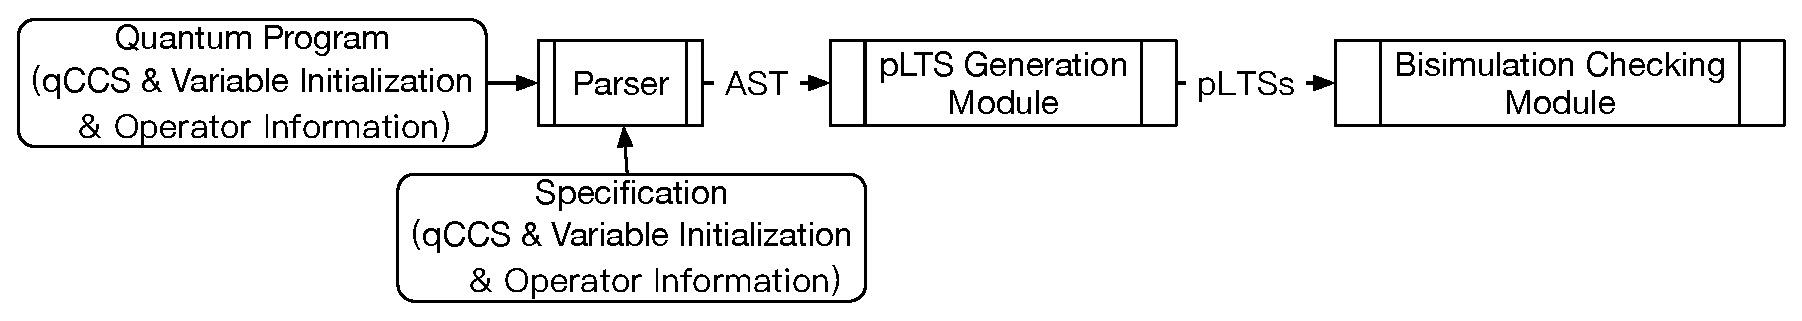
\includegraphics[width=\textwidth]{images/architecture.eps}
\caption{Verification workflow.}
\label{fig:arch}
\end{figure}
\begin{table}[htbp]
\centering
\begin{tabular}{@{}m{0pt}@{}
                >{\centering\arraybackslash}m{2cm}
                ||>{\centering\arraybackslash}m{3cm}
                |>{\centering\arraybackslash}m{1cm}
                |>{\centering\arraybackslash}m{0.8cm}
                |>{\centering\arraybackslash}m{0.8cm}
                |>{\centering\arraybackslash}m{0.8cm}
                |>{\centering\arraybackslash}m{0.8cm}
                |>{\centering\arraybackslash}m{1.1cm}}
\hline
\rule{0pt}{5mm}&\textbf{Program} & \textbf{Variables} & \textbf{Bisim} & \textbf{Impl} & \textbf{Spec} & \textbf{$N$} & \textbf{$B$} & \textbf{Sec} \\
\hline
\hline
\rule{0pt}{12mm}&Super-dense coding 1 & \tabincell{c}{$q_1=|0\rangle$\\$q_2=|0\rangle$\\$x=1$} & Yes & 15 & 15 & 0 & 11 & 11 \\
\hline
\rule{0pt}{12mm}&Super-dense coding 2 & \tabincell{c}{$q_1=|0\rangle$\\$q_2=|0\rangle$\\$x=5$} & No & 5 & 12 & - & - & 0.2 \\
\hline
\rule{0pt}{12mm}&Super-dense coding (modified) & \tabincell{c}{$q_1=|0\rangle$\\$q_2=|0\rangle$\\$x=5$} & Yes & 15 & 15 & 0 & 11 & 11 \\
\hline
\rule{0pt}{12mm}&Teleportation 1 & \tabincell{c}{$q_1=|1\rangle$\\$q_2=|0\rangle$\\$q_3=|0\rangle$} & Yes & 33 & 15 & 0 & 22 & 19 \\
\hline
\rule{0pt}{12mm}&Teleportation 2 & \tabincell{c}{$q_1=\frac{1}{\sqrt{2}}|0\rangle+\frac{1}{\sqrt{2}}|1\rangle$\\$q_2=|0\rangle$\\$q_3=|0\rangle$} & Yes & 33 & 15 & 0 & 22 & 19 \\
\hline
\rule{0pt}{12mm}&Teleportation 3 & \tabincell{c}{$q_1=\frac{\sqrt{3}}{2}|0\rangle+\frac{1}{2}|1\rangle$\\$q_2=|0\rangle$\\$q_3=|0\rangle$} & Yes & 33 & 15 & 0 & 22 & 19 \\
\hline
\rule{0pt}{15mm}&Secret Sharing 1 & \tabincell{c}{$q_1=|1\rangle$\\$q_2=|0\rangle$\\$q_3=|0\rangle$\\$q_4=|0\rangle$} & Yes & 102 & 26 & 0 & 65 & 62 \\
\hline
\rule{0pt}{15mm}&Secret Sharing 2 & \tabincell{c}{$q_1=\frac{1}{\sqrt{2}}|0\rangle+\frac{1}{\sqrt{2}}|1\rangle$\\$q_2=|0\rangle$\\$q_3=|0\rangle$\\$q_4=|0\rangle$} & Yes & 102 & 26 & 0 & 65 & 66 \\
\hline
\rule{0pt}{15mm}&Secret Sharing 3 & \tabincell{c}{$q_1=\frac{\sqrt{3}}{2}|0\rangle+\frac{1}{2}|1\rangle$\\$q_2=|0\rangle$\\$q_3=|0\rangle$\\$q_4=|0\rangle$} & Yes & 102 & 26 & 0 & 65 & 58 \\
\hline
\rule{0pt}{10mm}&BB84 & \tabincell{c}{$q1=|0\rangle$\\$q2=|0\rangle$} & Yes & 151 & 131 & 304 & 414 & 1371 \\
\hline
\rule{0pt}{12mm}&BB84 (with eavesdropper) & \tabincell{c}{$q1=|0\rangle$\\ $q2=|0\rangle$\\$q3=|0\rangle$} & No & 1243 & 763 & - & - & 56367 \\
\hline
\rule{0pt}{12mm}&BB84 (with eavesdropper \& modified) & \tabincell{c}{$q1=|0\rangle$\\$q2=|0\rangle$\\$q3=|0\rangle$} & Yes & 1179 & 779 & 17272 & 12294 & 1585740 \\
\hline
\end{tabular}
\vspace{1em}
\caption{Experimental Results. The
columns headed by \textbf{Impl} and \textbf{Spec} show the number of nodes contained in the generated pLTSs of implementation and specification. Column $N$ shows the size of the non-bisimilar pairs set $N$. Column $B$ shows the size of the bisimilar pairs set $B$. Column \textbf{SEC} shows verification
runtimes of the tool, times are in milliseconds.}\label{tab:result}  
\end{table}
\subsection{Examples: Quantum Communication Protocols}
We display four examples in our experiment:(1)Super-dense Coding Protocol; (2)Quantum Teleportation Protocol; (3)Quantum Secret Sharing; (4)BB84 Quantum Key Distribution Protocol. Firstly, we make a brief introduction about them. More details about them, including qCCS presentations are presented in Appendix~\ref{sec:examples}. 
\subparagraph*{Super-dense Coding Protocol.} There are two roles $Alice$ and $Bob$. To simplify the experiment, we only consider the smallest case of the protocol, sending only one qubit. So there is totally one entanglement on two qubits in this example. Besides the Clifford operators, we use a quantum operation $Set^{\Psi}$ to present the generation of EPR state whose operation elements are $\{|\beta_{00}\rangle\langle00|,|\beta_{00}\rangle\langle01|,|\beta_{00}\rangle\langle10|,|\beta_{00}\rangle\langle11|\}$ instead of using a combination of other quantum gates. The measurement used here is according to the computational basis $\{|00\rangle,|01\rangle,|10\rangle,|11\rangle\}$. The specification of the super-dense protocol is defined as $Bob$ sets the 2-qubit variable to the value according to the classical value he received from $Alice$.
\subparagraph*{Quantum Teleportation Protocol.} There are two roles in this example, similar with the last example. The operators we used here is also similar with the last example containing Clifford operators, $Set^{\Psi}$ and the measurement according to the same basis. However, we need one more entanglement and one more qubit even if we just consider the smallest case. The final result of this protocol we focus on is presented on the third qubit, $Bob's$ qubit. It should become the same value of the first qubit. So the specification of that can be presented by applying a \textit{SWAP} operation between the first and the third qubit.
\subparagraph*{Quantum Secret Sharing.} In this example, there are three roles. The operators used here are almost the operators we have used in teleportation protocol except that we use a quantum operation $Set^{GHZ}$ to present the generation of 3-qubit maximally entangled states. This example is closed to the teleportation example, the difference is that it makes four qubits entangled together. So its specification becomes applying a \textit{SWAP} operation between the first and the fourth qubit.
\subparagraph*{BB84 Quantum Key Distribution Protocol.} In BB84 protocol, there is no entanglement at all, its method needs generating qubits on different basis and using different measurement method without any contacts in advance with the other side. If someone tries intercepting the information, the qubits might be measured in wrong basis, it brings a possibility that $Alice$ and $Bob$ can be aware of the attack. So the protocol uses one more kind of measurement which is according to the diagonal basis $\{|+\rangle,|-\rangle\}$. In common use case, BB84 will send a sequence of the qubits while qubits will not influence each other. We consider two kinds of result of the communication. First case is that $Alice$ and $Bob$ choose the same measurement then the results they get are also the same. Another case is that they choose different measurements then the result is discarded at this time. In the specification, we get results from the same sequence instead of two result sequence separately. Considering results from both sides is always the same, this operation will not bring any difference.
\subparagraph*{BB84 Protocol with an Eavesdropper.} This example is an extension of the BB84 example, supposing there is an eavesdropper attending into the communication. There have three roles and the new role $Eve$ also randomly choose the measurement just as what $Alice$ and $Bob$ do. The specification is also similar with the one without an eavesdropper. It is possible that the eavesdropper will be recognized. It is a new result of the program. We conclude these results into three messages: emitting through the channel $alarm$ as the measurement methods are not matched; emitting through the channel $fail$ as the measurement methods are matched while the eavesdropping is recognized; normal emitting as the communication finished without recognizing the eavesdropper.
\subsection{Experimental Results}
We conducted experiments on those quantum communication protocols and obtained the results  on a macOS machine with an Intel Core i7 2.5 GHz processor and 16GB of RAM.
\subparagraph*{Experimental Results and Improvement.}Table~\ref{tab:result} provides a summary of our experimental results over those four examples. In each case, we report the bisimilarity, the number of nodes in two pLTSs, the number of non-bisimilar and bisimilar states pair in $N$, $B$ and the runtime of our checking algorithm (not including the pLTS generation part).

We verify the super-dense coding with two different initial valuations of variable $x$ in the first two lines. In the case $x=1$, we can check that protocol and its specification are bisimilar. However, in the case $x=5$, when none of the four branches is chosen, they are not bisimilar because of the different length of the trace. The result shows that the program misses the solution for the valuation out of the expected scale. We improve the program through adding a new branch solving all the unexpected value. The result of the improved program is presented on the third line. 

We also verify the teleportation with several different initial valuations of qubits. The input qubits are used to generate the EPR state or other fixed value in other examples, what is different from this example. The qubit $q_1$ in the inputs decides the final state of the qubit $q_3$. We can find that there is no difference between the result information from different inputs.

Another example brings a non-bisimilarity is on the second line from the bottom, which is the BB84 protocol considering the eavesdropper. $Alice$ and $Bob$ will make an alert if their measurement methods are not matched. The parallelism between the final test process and them leads to the process continues behaving some actions. That is not what the specification exactly describes. To improve this program, we modify the behavior, move the alert to the test process. $Alice$ and $Bob$ only send messages when they find they use different measurements. As a result, on the last line of the table, we find the program is bisimilar with the specification.
\subparagraph*{Discussion.} Not all the cases of Table~\ref{tab:result} present the size of the non-bisimilar states set $N$, as the checking algorithm has terminated at an early point. Furthermore, to ensure the bisimilarity between program with a large set of states and its specification requires much more time, over tens of times more than the runtime of checking non-bisimilarity. However, the runtime of finding two pLTSs are non-bisimilar is not that long enables us to try making improvement in an acceptable time waiting feedback.

\section{Conclusion and Future Works}
In this paper we have presented an on-the-fly algorithm verifying strong ground bisimulation for quantum programs in qCCS. And then we have developed a tool for bisimilarity checking basing on the algorithm. The input is encoded with the notation of qCCS, which enables us to translate the program to corresponding finite pLTS depending on its operational semantics. We proved our algorithm terminates on checking two finite tree-structural pLTSs and figures out the bisimilarity. To show its performance, we further made experiments on several quantum communication protocols such as BB84. The experimental results have showed the algorithm is able to provide hints for two kinds of improvement: (1) supplementing the missing cases of the programs; (2) adjusting how the parallel behaviours collaborate with each other.

There are still many questions remaining for further study.Firstly, the bisimulation checking may not only several possible inputs which we can enumerate all of them in a short time. One of the solution of that is to introduce the idea of symbolic bisimulation proposed in~\cite{FDY14}. Symbolic bisimulation uses an accumulation of the super-operators instead of a density operator to present the state which allows us to verify the programs with arbitrary inputs. However, the normalizing operation is also unavailable without the density operator, so it becomes a challenge.

Secondly, it is eye-catching that there are too many invisible action $\tau$ contained in the programs especially the specification programs matching the internal communications and quantum operations in the implementation programs. To deal with this problem, we are going to implement a weak bisimulation checking algorithm wipe out those invisible actions. 

%%
%% Bibliography
%%

%% Please use bibtex, 

%\bibliographystyle{abbrv}
\bibliography{ref}

\appendix

\section{Examples in qCCS}
\label{sec:examples}
\subsection{Super-dense Coding Protocol}
Super-dense coding is proposed by Bennett and Wiesner in 1992~\cite{BW92}. It is a quantum communication protocol allowing two classical bits to be encoded in one qubit during a transmission, so it needs only one quantum channel. Such advantage bases on the use of a maximally
entangled state, EPR state. An EPR state can be transformed into all the four kinds of EPR states through an one-qubit operation, and these EPR states are mutually orthogonal. We suppose the sender and the receiver of the communication are $Alice$ and $Bob$, then the protocol goes as follows:
\begin{bracketenumerate}
    \item $Alice$ and $Bob$ prepare an EPR state $|\beta_{00}\rangle_{q_1,q_2}$ together. Then they share the qubits, $Alice$ holding $q_1$ and $Bob$ holding $q_2$.
    \item If $Alice$ wants to send value $x\in \{0,1,2,3\}$, she applies the corresponding Pauli operation $\sigma^{x}$ on her qubit $q_1$.
    \item $Alice$ sends the qubit $q_1$ to $Bob$.
    \item $Bob$ applies a controlled-not operation on $q_1,q_2$ and a Hadamard operation on $q_1$ to remove the entanglement.
    \item $Bob$ measures $q_1$ and $q_2$ to get the value $x$.
\end{bracketenumerate}
After the execution of the protocol above, $Bob$ gets the value $x$ which $Alice$ wants to send. Considering $x$ could be presented in a two-bit string, the protocol exactly transmits two classical bits of information by sending one qubit from $Alice$ to $Bob$.
\subparagraph*{Implementation.}
Now we design the program of super-dense coding protocol in qCCS as follows:
\begin{flalign*}
    Alice \overset{def}{=}& \underline{c}_{A}?q_1.\sum_{0\leq  i\leq 3}(\textbf{if}\ x=i\ \textbf{then}\ \sigma^{i}[q_1].\underline{e}!q_1.\textbf{nil});\\
    Bob \overset{def}{=}& \underline{c}_{B}?q_2.\underline{e}?q_1.\mathcal{CN}[q_1,q_2].\mathcal{H}[q_1].M[q_1,q_2;x].d!x.\textbf{nil};\\
    EPR \overset{def}{=}& Set^{\Psi}[q_1,q_2].\underline{c}_{B}!q_2.\underline{e}_{A}!q_1.\textbf{nil};\\
    Sdc \overset{def}{=}& c?x.(Alice||Bob||EPR)\setminus \{\underline{c}_{A},\underline{c}_{B},\underline{e}\}
\end{flalign*}
where $\mathcal{CN}$ is the controlled-not operation and $\mathcal{H}$ is the Hadamard operation, $Set^{\Psi}$ is the operation transforming all the inputs into an EPR state $|\beta_{00}\rangle=(|00\rangle+|11\rangle)/\sqrt{2}$, its operation elements are $\{|\beta_{00}\rangle\langle 00|,|\beta_{00}\rangle\langle 01|,|\beta_{00}\rangle\langle 10|,|\beta_{00}\rangle\langle 11|\}$, and $\sigma^{i}$ are Pauli operators where $\sigma^{0}=I,\sigma^{1}=X,\sigma^{2}=Z,\sigma^{3}=Y$. The element set of measurement \textit{M} is $\{|00\rangle\langle 00|,|01\rangle\langle 01|,|10\rangle\langle 10|,|11\rangle\langle 11|\}$.
\subparagraph*{Specification.}
The specification of super-dense coding protocol can be defined as:
\begin{flalign*}
    Sdc_{spec} \overset{def}{=}& c?x.\tau^{11}.\sum_{i=0}^{3}(\textbf{if}\ x=i\ \textbf{then}\ Set^{i}[q_1,q_2].d!x.\textbf{nil})
\end{flalign*}
where $Set^{i}$ is the operation transforming the current state into the state decided by the value of $i$ like $Set^{\Psi}$.
\subparagraph*{Improved Super-dense Coding Protocol.}
We improve the program through adding an extra solution for the value $i\neq 1,2,3,4$. We send a message alarming we have encountered such case and skip all the rest operations. The new program of $Sdc$ is:
\begin{flalign*}
    Alice \overset{def}{=}& \underline{c}_{A}?q_1.(\sum_{0\leq  i\leq 3}(\textbf{if}\ x=i\ \textbf{then}\ \sigma^{i}[q_1].\underline{e}!q_1.\textbf{nil})\ \\
    & +\ \textbf{if}\ \neg\bigvee_{0\leq  i\leq 3} x=i\ \textbf{then}\ c_{C}!msg.\textbf{nil});\\
    Bob \overset{def}{=}& \underline{c}_{B}?q_2.(\underline{e}?q_1.\mathcal{CN}[q_1,q_2].\mathcal{H}[q_1].M[q_1,q_2;x].d!x.\textbf{nil}\ +\ c_{C}?msg.\tau^{8}.d!x.\textbf{nil});\\
    EPR \overset{def}{=}& Set^{\Psi}[q_1,q_2].\underline{c}_{B}!q_2.\underline{c}_{A}!q_1.\textbf{nil};\\
    Sdc \overset{def}{=}& c?x.(Alice||Bob||EPR)\setminus \{\underline{c}_{A},\underline{c}_{B},c_{C},\underline{e}\}.
\end{flalign*}
And we adjust the specification as the program has a new branch, so it is defined as:
\begin{flalign*}
    Sdc_{spec} \overset{def}{=}& c?x.\tau^{11}.\sum_{i=0}^{3}(\textbf{if}\ x=i\ \textbf{then}\ Set^{i}[q_1,q_2].d!x.\textbf{nil})\\
    &\ +\ \textbf{if}\ \neg\bigvee_{0\leq  i\leq 3} x=i\  \textbf{then}\ Set^{\Psi}[q_1,q_2].d!x.\textbf{nil}).
\end{flalign*}
\subsection{Quantum Teleportation Protocol}
Quantum teleportation~\cite{BB93} is one of the most important protocols in quantum information theory. It teleports an unknown quantum state by only sending  classical information, so it just requires a classical communications channel. It makes the use of the maximally entangled states that the post-measurement state can be known from the result of partial measurement for a set of entangled states. Let sender and receiver to be $Alice$ and $Bob$ as defined in super-dense coding example, the quantum teleportation protocol goes as follows:
\begin{bracketenumerate}
    \item $Alice$ and $Bob$ prepare an EPR state $|\beta_{00}\rangle_{q_2,q_3}$ together. Then they share the qubits, $Alice$ holding $q_2$ and $Bob$ holding $q_3$.
    \item To transmit qubit $q_1$, $Alice$ applies a $\mathcal{CN}$ operation on $q_1$ and $q_2$ followed by a $\mathcal{H}$ operation on $q_1$.
    \item $Alice$ measures $q_1$ and $q_2$ and sends the outcome $x$ to $Bob$.
    \item $Bob$ applies corresponding $\sigma^{x}$ operation on his qubit $q_3$ to recover the original state of $q_1$.
\end{bracketenumerate}
After the execution, $Bob's$ qubit $q_3$ has the same state as the qubit $q_1$.
\subparagraph*{Implementation.}
The program of quantum teleportation protocol can be encoded in qCCS as follows:
\begin{flalign*}
    Alice \overset{def}{=}& \underline{c}_{A}?q2.\mathcal{CN}[q_1,q_2].\mathcal{H}[q_1].M[q_1,q_2;x].Set^{\Psi}[q_1,q_2].e!x.\textbf{nil};\\
    Bob \overset{def}{=}& \underline{c}_{B}?q_3.e?x.\sum_{0\leq i\leq 3}(\textbf{if}\ x=i\ \textbf{then}\ \sigma^{i}[q_3].\textbf{nil});\\
    EPR \overset{def}{=}& Set^{\Psi}[q_1,q_2].\underline{c}_{A}!q_2.\underline{c}_{B}!q_3.\textbf{nil};\\
    Tel \overset{def}{=}& (Alice||Bob||EPR)\setminus \{\underline{c}_{A},\underline{c}_{B},e\}
\end{flalign*}
where the operators used are all already declared before. 
\subparagraph*{Specification.}
The specification of quantum teleportation protocol can also be described in qCCS. To show the soundness of $Tel$, it suffices to prove that $Tel$ is bisimilar to an swap operation between the first and the thrid qubits, that is $\mathcal{SWAP}_{1,3}[q_1,q_3]$. The program can be encoded as follow:
\begin{flalign*}
    Spec &\overset{def}{=} \tau^{13}.\mathcal{SWAP}[q_1,q_3].\textbf{nil}.
\end{flalign*}
\subsection{Quantum Secret Sharing Protocol}
Quantum Secret Sharing Protocol is first developed by Hillery et al.~\cite{hillery1999quantum}. The problem involves an agent $Alice$ sending information to other two agents $Bob$ and $Charlie$ one of whom is dishonest. It is a classical method which is known as secret sharing that $Alice$ split the information into two parts, then $Bob$ and $Charlie$ need collaboration to get the complete information. It lets the honest one keep the dishonest one from doing damage. A quantum version of it can be realized by a three-qubit maximally entangled state called GHZ state, which has similar property as EPR state. The protocol goes as follows:
\begin{bracketenumerate}
    \item $Alice$, $Bob$ and $Charlie$ prepare an GHZ state $(|000\rangle+|111\rangle)/\sqrt{2}_{q_2,q_3,q_4}$ together prior to the following execution. Then they share the qubits, $Alice$ holding $q_2$, $Bob$ holding $q_3$ and $Charlie$ holding $q_4$.
    \item $Alice$ entangles $q_1$ and $q_2$ applying a $\mathcal{CN}$ operation followed by a $\mathcal{H}$ operation on $q_1$.
    \item $Alice$ measures $q_1$ and $q_2$ separately and sends the outcomes $m$ and $n$ to $Charlie$.
    \item $Bob$ also measures $q_3$ and sends the outcome $o$ to $Charlie$.
    \item Upon receiving the bits $m$, $n$ and $o$, $Charlie$ retrieves the state through applying Pauli operations $\mathcal{X}$ or $\mathcal{Z}$ on $q_4$ according to the value of these bits.
\end{bracketenumerate}
After the execution, $Charlie's$ qubit $q_4$ has the same state as the qubit $q_1$.
\subparagraph*{Implementation.}
The program of quantum teleportation protocol can be encoded in qCCS as follows:
\begin{flalign*}
    Alice \overset{def}{=}& \underline{c}_{A}?q2.\mathcal{CN}[q_1,q_2].\mathcal{H}[q_1].M[q_1;m].M[q_2;n].e!m.f!n.\textbf{nil};\\
    Bob \overset{def}{=}& \underline{c}_{B}?q_3.\mathcal{H}[q_2].M[q_2;o].g!o.\textbf{nil});\\
    Charlie \overset{def}{=}& \underline{c}_{C}?q_4.e?m.f?n.g?o.\\
    &\textbf{if}\ o=1\ \textbf{then}\ \mathcal{Z}[q_4].\textbf{if}\ m=1\ \textbf{then}\ \mathcal{X}[q_4].\textbf{if}\ n=1\ \textbf{then}\ \mathcal{Z}[q_4].\textbf{nil});\\
    GHZ \overset{def}{=}& Set^{GHZ}[q_2,q_3,q_4].\underline{c}_{A}!q_2.\underline{c}_{B}!q_3.\underline{c}_{C}!q_4.\textbf{nil};\\
    QSS \overset{def}{=}& (Alice||Bob||Charlie||GHZ)\setminus \{\underline{c}_{A},\underline{c}_{B},\underline{c}_{C},e,f,g\}
\end{flalign*}
where the operators used are all already declared before except that $Set^{GHZ}$ is the operation transforming all the inputs into an GHZ state which is similar with $Set^{\Psi}$.
\subparagraph*{Specification.}
To show its soundness, we prove that $QSS$ is bisimilar to an swap operation between the first and the fouth qubits, that is $\mathcal{SWAP}_{1,4}[q_1,q_4]$. The program can be encoded as follow:
\begin{flalign*}
    Spec &\overset{def}{=} \tau^{24}.\mathcal{SWAP}[q_1,q_4].\textbf{nil}.
\end{flalign*}
\subsection{BB84 Quantum Key Distribution Protocol}
BB84 is the first quantum key distribution protocol developed by Bennett and Brassard in
1984~\cite{BB84}. It provides a provably secure way to create a private key between two partners with a classical authenticated channel and a quantum insecure
channel between them. The protocol does not make the use of entangled states. It ensures its security through the basic property of quantum mechanics: if the states to be distinguished are not orthogonal, such as $|0\rangle$ and $|+\rangle$, then information gain about a quantum state is only
possible at the expense of changing the state. Let sender and receiver to be $Alice$ and $Bob$ as defined in previous examples, the basic BB84 protocol with a sequence of qubits $\tilde{q}$ with size $n$ goes as follows:
\begin{bracketenumerate}
    \item $Alice$ randomly generates two sequences of bits $\tilde{B}_a$ and $\tilde{K}_a$ using her qubits $\tilde{q}$.
    \item $Alice$ prepares the state of $\tilde{q}$, such that the \textit{i}th bits of $\tilde{q}$ is $|x_{y}\rangle$ where $x$ and $y$ are the \textit{i}th bits of $\tilde{B}_a$ and $\tilde{K}_a$, and respectively,  $|0_0\rangle=|0\rangle$, $|0_1\rangle=|1\rangle$, $|1_0\rangle=|+\rangle=(|0\rangle+|1\rangle)/\sqrt{2}$ and $|1_1\rangle=|-\rangle=(|0\rangle-|1\rangle)/\sqrt{2}$.
    \item $Alice$ sends her qubits $\tilde{q}$ to $Bob$.
    \item $Bob$ randomly generates a sequence of bits $\tilde{B}_b$ using his qubits $\tilde{q'}$.
    \item $Bob$ measures the \textit{i}th qubit of $\tilde{q}$ he received from $Alice$ according to the basis determined by the \textit{i}th bit of $\tilde{B}_b$. Respectively, the basis is $\{|0\rangle,|1\rangle\}$ if it is $0$ and $\{|+\rangle,|-\rangle\}$ if it is $1$.
    \item $Bob$ sends his choice of measurements $\tilde{B}_{b}$ to $Alice$, and after receiving the information, $Alice$ sends her $\tilde{B}_{a}$ to $Bob$.
    \item $Alice$ and $Bob$ match two sequences of bits $\tilde{B}_{a}$ and $\tilde{B}_{b}$ to determine at which positions the bits are equal. If the bits match, they keep the corresponding bits of $\tilde{K}_a$ and $\tilde{K}_b$. Otherwise, they discard them.
\end{bracketenumerate}
After execution the basic BB84 protocol, the remaining bits of $\tilde{K}_a$ and $\tilde{K}_b$ should be the same, provided that the communication channels are prefect and there is no eavesdropper.

Then we consider the case that there exists an eavesdropper called $Eve$ taking part in the communication. $Alice$ and $Bob$ also have more behaviours to detect $Eve$. In the BB84 protocol with eavesdropper, let $\tilde{K'}_a$ and $\tilde{K'}_b$ to be the remaining bits of $\tilde{K}_a$ and $\tilde{K}_b$ with size $k$, $Eve$, $Alice$ and $Bob$ proceed as follows:
\begin{bracketenumerate}
    \item $Alice$ randomly chooses $\lceil k/2\rceil$ bits of $\tilde{K'}_a$, denoted by $\tilde{K''}_a$ and sends it to $Bob$ together with the indexes of the chosen bits.
    \item After receiving the information from $Alice$, $Bob$ chooses $\lceil k/2\rceil$ bits of $\tilde{K'}_b$ according to the indexes he received, denoted by $\tilde{K''}_b$ and sends it back to $Alice$.
    \item $Alice$ and $Bob$ match two sequences of bits $\tilde{K''}_{a}$ and $\tilde{K''}_{b}$. If two sequences match, then they have not detected the eavesdropper and the remaining substring of $\tilde{K'}_{a}$ and $\tilde{K'}_{b}$ are used as the secure key. Otherwise, they detect $Eve$ and the protocol halts without generating any secure keys.
\end{bracketenumerate}

\subparagraph*{Implementation.}
The program we written here only contains one qubit instead of a sequence of qubits, however, it is enough to reflect all the cases could occur. The other qubits used here are auxiliary qubits for $Ran$ operation.
\begin{flalign*}
    Alice \overset{def}{=}& Ran[q_1;B_{a}].Ran[q_1;K_{a}].Set_{K_{a}}[q_1].H_{B_{a}}[q_1].\underline{A2B}!q_1.\\ 
    &\qquad\qquad\qquad b2a?B_{b}.a2b!B_{a}.key_{a}!cmp(K_{a},B_{a},B_{b}).\textbf{nil};\\
    Bob \overset{def}{=}& \underline{A2B}?q_1.Ran[q_2;B_{b}].M_{B_{b}}[q_1;K_{b}].b2a!B_{b}.\\
    &\qquad\qquad\qquad a2b?B_{a}.key_{b}!cmp(K_{b},B_{a},B_{b}).\textbf{nil};\\
    BB84 \overset{def}{=}& (Alice||Bob)\setminus\{a2b,b2a,\underline{A2B}\}
\end{flalign*}
where there are several special operations:
\begin{itemize}
    \item $Ran[q;x]=Set_{+}[q].M_{0,1}[q;x].Set_{0}[q]$, where $Set_{+}$ (resp.$Set_{0}$) is the operation which sets a qubit it applies on to $|+\rangle$ (resp.$|0\rangle$), $M_{0,1}[q;x]$ is the quantum measurement on $q$ according to the basis $\{|0\rangle,|1\rangle\}$ and stores the result into $x$.
    \item $Set_{K}[q]$ sets the qubit $q$ to the state $|K\rangle$.
    \item $H_{B}[q]$ applies $H$ or does nothing on the qubit $q$ depending on whether the value of $B$ is 1 or 0.
    \item $M_{B}[q;K]$ is the quantum measurement on $q$ according to the basis $\{|+\rangle,|-\rangle\}$ or $\{|0\rangle,|1\rangle\}$ depending on whether the value of $B$ is 1 or 0.
    \item $cmp(x,y,z)$ returns $x$ if $y$ and $z$ match, and $\epsilon$, meaning it is empty, if they do not match.
\end{itemize}
\subparagraph*{Specification.}
Its specification can be defined as follow using the same operations:
\begin{flalign*}
    BB84_{spec} \overset{def}{=}& Ran[q_1;B_{a}].Ran[q_1;K_{a}].Ran[q_2;B_{b}]\\
    &\qquad\qquad\qquad.(key_{a}!cmp(K_{a},B_{a},B_{b}).\textbf{nil}||cmp(K_{b},B_{a},B_{b}).\textbf{nil}).
\end{flalign*}

\subparagraph*{Implementation with an Eavesdropper.}
Then we proceed to describe the protocol with an eavesdropper. We extend the processes $Alice$ and $Bob$ with a process for eavesdropper detection.
\begin{flalign*}
    Alice' \overset{def}{=}& key_{a}?K'_{a}.Pstr_{K'_{a}}[q_1;x].a2b!x.a2b!SubStr(K'_{a},x).b2a?K''_{b}.\\
    &(\textbf{if}\ SubStr(K'_{a},x)=K''_{b}\ \textbf{then}\ key'_{a}!RemStr(K'_{a},x).\textbf{nil} \\
    &\textbf{else}\ alarm_{a}!0.\textbf{nil});\\
    Bob' \overset{def}{=}& key_{b}?K'_{b}.a2b?x.a2b?K''_{a}.b2a!SubStr(K'_{b},x).\\
    &(\textbf{if}\ SubStr(K'_{b},x)=K''_{a}\ \textbf{then}\ key'_{b}!RemStr(K'_{b},x).\textbf{nil} \\
    &\textbf{else}\ alarm_{b}!0.\textbf{nil})
\end{flalign*}
where there are three more special operations:
\begin{itemize}
    \item $Pstr$ is a measurement which is similar to $Ran$, randomly generates the value of $x$.
    \item $SubStr(K,x)$ returns the substring of K at the index specified by $x$.
    \item $RemStr(K,x)$ returns the remaining substring of K by deleting $SubStr(K,x)$.
\end{itemize}
After that, we give the definition of the eavesdropper:
\begin{flalign*}
    Eve \overset{def}{=}& \underline{A2E}?q_1.Ran[q_3;B_{e}].M_{B_{e}}[q_1;K_{e}].Set_{K_{e}}[q_1].H_{B_{e}}[q_1].\underline{E2B}!q_1.key_{e}!K_{e}.\textbf{nil}.
\end{flalign*}
With the attending of $Eve$, we adjust the communication of $Alice$ and $Bob$:
\begin{flalign*}
    Alice\longrightarrow Alice[f_{a}], Bob\longrightarrow Bob[f_{b}]
\end{flalign*}
where $f_{a}(\underline{A2B})=\underline{A2E}$, and $f_{b}(\underline{A2B})=\underline{E2B}$.

We use a test process to conclude the final result:
\begin{flalign*}
    Test \overset{def}{=}& key'_{a}?x.key'_{b}?y.key'_{e}?z.\\
    &(\textbf{if}\ x\neq y\ \textbf{then}\  fail!0.\textbf{nil}\\
    &\ +\ \textbf{if}\ x=y\ \textbf{then}\ key_{e}!z.skey!x.\textbf{nil});\\
    BB84 \overset{def}{=}& (Alice||Bob||Alice'||Bob'||Eve||Test)\setminus C
\end{flalign*}
where $C=\{a2b,b2a,key_{a},key_{b},\underline{A2E},\underline{E2B},alarm_{a},alarm_{b}\}$.
\subparagraph*{Specification.}
The specification of that can be defined as:
\begin{flalign*}
    Spec \overset{def}{=}& Ran[q_1;B_{a}].Ran[q_1;K_{a}].Ran[q_3;B_{e}].Ran'_{B_{a},B_{e},K_{a}}[q_1;K_{e}].Ran[q_2;K_{b}].\\
    &Ran'_{B_{e},B_{b},K_{e}}[q_1;K_{b}].Pstr_{}[q_1;x].\\
    &(\textbf{if}\ K_{ab}=K_{ba}\ \textbf{then}\ key_{e}!K_{e}.skey!RemStr(K_{ab},x).\textbf{nil}\\
    &\ + \textbf{if}\ K_{ab}\neq K_{ba}\ \textbf{then}\\
    &\ (\textbf{if}\ K^{x}_{ab}\neq K^{x}_{ba}\ \textbf{then}\ alarm_{a}!0.\textbf{nil}||alarm_{b}!0.\textbf{nil}\\
    &\ +\ \textbf{if}\ K^{x}_{ab}=K^{x}_{ba}\ \textbf{then}\ fail!0.\textbf{nil}))
\end{flalign*}
where $K_{ab}=cmp(K_{a},B_{a},B_{b})$,  $K_{ba}=cmp(K_{b},B_{a},B_{b})$, $K^{x}_{ab}=SubStr(K_{ab},x)$, $K^{x}_{ab}=SubStr(K_{ba},x)$. And similar to $Ran$, $Ran'_{x,y,z}[q;v]$ is a special measurement randomly generate the value of $v$ if $x$ and $y$ do not match and give $v$ the value of $z$ if they match.

\subparagraph*{Improved BB84 Protocol with an Eavesdropper.}
As the reason why the problem occurred is that the operation $alarm$ is not concluded in $Test$ and the implementation have more behaviours than what the specification requires. So we only refine the program of implementation, adding a message communication with $Test$:
\begin{flalign*}
    Alice' \overset{def}{=}& key_{a}?K'_{a}.Pstr_{K'_{a}}[q_1;x].a2b!x.a2b!SubStr(K'_{a},x).b2a?K''_{b}.\\
    &(\textbf{if}\ SubStr(K'_{a},x)=K''_{b}\ \textbf{then}\ key'_{a}!RemStr(K'_{a},x).\textbf{nil} \\
    &\textbf{else}\ msg_{a}!0.\textbf{nil});\\
    Bob' \overset{def}{=}& key_{b}?K'_{b}.a2b?x.a2b?K''_{a}.b2a!SubStr(K'_{b},x).\\
    &(\textbf{if}\ SubStr(K'_{b},x)=K''_{a}\ \textbf{then}\ key'_{b}!RemStr(K'_{b},x).\textbf{nil} \\
    &\textbf{else}\ msg_{b}!0.\textbf{nil});\\
    Test \overset{def}{=}& key'_{a}?x.key'_{b}?y.key'_{e}?z.\\
    &(\textbf{if}\ x\neq y\ \textbf{then}\  fail!0.\textbf{nil}\ +\ \textbf{if}\ x=y\ \textbf{then}\ key_{e}!z.skey!x.\textbf{nil})\\
    &+\ msg_{a}?x.msg_{b}?y.key'_{e}?z.alarm!0.\textbf{nil}.
\end{flalign*}

\section{Proving Correctness of the Ground Algorithm}
\label{sec:correctness}
% \begin{lemma}
% 	Todo: prove that we can ensure in such case, the trace is  longer than any other trace from another side or unmatched with them.
% \end{lemma}
% \begin{theorem}[Early termination]
% 	If the algorithm reaches a leaf state of the tree-like pLTS while the state of the other pLTS is not a leaf state, then these two pLTSs are not bisimilar.
% \end{theorem}
% \begin{proof}
% 	We consider it on the aspect of the length of the traces. From the structure of the algorithm, each time \textbf{MatchAction} is called \textbf{Act} will be called before it. So we can ensure that two states have the same action to behave. There exists the trace that
% 	\[T = \langle t_0,\rho\rangle\xrightarrow{\gamma_0}...\xrightarrow{\gamma_i}\langle t_i,\rho\rangle\text{ and }U = \langle u_0,\sigma\rangle\xrightarrow{\gamma_0}...\xrightarrow{\gamma_i}\langle u_i,\sigma\rangle.\]
% 	Let $|T|=|U|=n$, if one of these states $u_i$ is not a leaf, then there has a longer trace $|U'|=n+1$. As there is no loop contained, the trace $|T'|=n+1$ does not exist, so we can not find a trace has the same length as that one. According to the definition of the bisimulation, these two pLTS should not satisfy it.
% \end{proof}

In this appendix, we consider the correctness of the algorithm. To simplify the presentation, we use \texttt{R}$(t,u,W,N)$ to mean the following condition is satisfied:
\begin{itemize}
    \item If $(t',u')\notin N\wedge t'\xrightarrow{\alpha}t''\wedge u'\xrightarrow{\alpha'}u'', (t',u')\notin\{(t,u)\}\cup W\wedge$: 
    % \item If $(t',u')\notin N$, then $\forall t'\xrightarrow{\alpha}t'',\exists u'\xrightarrow{\alpha'}u''$ and $(t'',u'')\notin \{(t,u)\}\cup W$ such that: 
    \begin{itemize}
        \item if $\alpha\equiv c!e\wedge\alpha'\equiv c!e'$ with $e=e'$, then $(t'',u'')\notin W\wedge(t'',u'')\notin N\implies t''\sim u''$.
        \item let $t''\equiv \Delta'$ and $u''\equiv \Theta'$, if $\alpha\equiv \tau\wedge\alpha'\equiv \tau$, then $\exists t'_i\in \lceil\Delta'\rceil, u'_j\in \lceil\Theta'\rceil,\ (t'_i,u'_j)\notin W\wedge(t'_i,u'_j)\notin N\implies t'_i\sim u'_j$.
        \item otherwise $\alpha=\alpha'$, then  $(t'',u'')\notin W\wedge(t'',u'')\notin N\implies t''\sim u''$.
    \end{itemize}
\end{itemize}

\begin{lemma}\label{lem:n_merge}
If $N_1\cap N_2=\emptyset$ then \texttt{R}$(t,u,W,N_1)$ and \texttt{R}$(t,u,W,N_2)$ $implies$ \texttt{R}$(t,u,W,N_1\cup N_2)$.
\end{lemma}
\begin{proof}
Straightforward from the definition of \texttt{R}.
\end{proof}

We define the verification conditions of our three matching functions.
\begin{definition}\label{def:match}
\textbf{Match}$(t,u,W)$ is \textit{true} if the following conditions ar satisfied:
\begin{itemize}
    \item(C1) $W\cap N=\emptyset$ and
    \begin{itemize}
        \item if $(t,u)\in W$, then $(t,u)\notin N$,
        \item if $(t,u)\notin W$, then either $\theta=true\wedge(t,u)\notin N$ or $\theta=false\wedge(t,u)\in N$.
    \end{itemize}
    \item(C2) $\texttt{R}(t,u,W,N)$.
\end{itemize}
Let \textbf{Bisim}$(t,u)=$\textbf{Match}$(t,u,\emptyset)$.
\end{definition}

\begin{definition}\label{def:matchaction}
\textbf{MatchAction}$(\gamma,t,u,W)$ is \textit{true} if all the following conditions are satisfied:
\begin{itemize}
    \item(M1) $W\cap N=\emptyset$, $(t,u)\notin W$ and $(t,u)\notin N$.
    \item(M2) $\texttt{R}(t,u,W,N)$.
    \item(M3) $\forall t\xrightarrow{\alpha}t', \exists u\xrightarrow{\alpha'}u'$, $(t',u')\notin \{(t,u)\}\cup W$ and 
    \begin{itemize}
        \item if $\alpha\equiv a$ (including $c?x$) then $\alpha'\equiv a$ and $(t',u')\notin W\wedge(t',u')\notin N\implies t'\sim u'$.
        \item if $\alpha\equiv c!e$ then $\alpha'\equiv c!e'$ with $e=e'$ and $(t',u')\notin W\wedge(t',u')\notin N\implies t'\sim u'$.
        \item let $t'\equiv \Delta$ and $u'\equiv \Theta$, if $\alpha\equiv \tau$ then $\alpha'\equiv \tau$, $\forall t_i\in \lceil\Delta\rceil, u_j\in \lceil\Theta\rceil,\ (t_i,u_j)\notin W\wedge(t_i,u_j)\notin N\implies t_i\sim u_j$.
    \end{itemize}
\end{itemize}
\end{definition}

\begin{definition}\label{def:matchdistribution}
\textbf{MatchDistribution}$(\Delta,\Theta,W)$ is \textit{true} if the following conditions are satisfied:
\begin{itemize}
    \item(D1) $W\cap N=\emptyset$, $\forall t_i\in \lceil\Delta\rceil, u_j\in \lceil\Theta\rceil,\ (t_i,u_j)\notin W$ and $\exists (t_i,u_j)\notin N$.
    % and $(t_i,u_j)\notin N\implies t_i\sim u_j$
    \item(D2) Let $t\xrightarrow{\alpha}\Delta, u\xrightarrow{\alpha'}\Theta$, $\texttt{R}(t,u,W,N)$.
\end{itemize}
\end{definition}

\begin{proposition}Let $\textbf{MatchAction}_\gamma(\gamma,t,u,W)$ is the execution of \textbf{MatchAction} with action $\gamma$.
If $\textbf{MatchAction}_\gamma(\gamma,t,u,W)$ is $true$ for each action $\gamma$ then \textbf{Match}$(t,u,W)$ is also $true$, where it returns $\theta=\bigwedge_\gamma\theta_\gamma$ and $N=\bigcup_\gamma N_\gamma$.
\end{proposition}
\begin{proof}
The only time point that $(t,u)$ is added into $W$ is during the execution of \textbf{MatchAction}, then according to the Definition~\ref{def:matchaction}, we have $W\cap N=\emptyset$. Since the verified pLTS is a finite tree, if they reach the leaf states of the pLTSs, there should have $\theta=true$ and $N=\emptyset$, at the same time it satisfies that $(t,u)\notin W\wedge(t,u)\notin N$. Furthermore, we have $t\sim u$ in such case. According to the structure of the function, $(t,u)$ will be added in to $N$ if $\theta$ is false. Overall, $C1$ is satisfied.

From condition (M2) and (M3), \texttt{R}$(t,u,W,N_{\gamma})$ exists. According to Lemma~\ref{lem:n_merge}, we have the condition that \texttt{R}$(t,u,W,\bigcup_{\gamma}N_{\gamma})$, it satisfies $C2$.
\end{proof}

\begin{proposition} Suppose $(t,u)\notin W$.
If \textbf{Match}$(t_i,u_j,W\cup\{(t,u)\})$ is $true$ for all actions $\gamma\neq\tau$ where exists transitions $(t\xrightarrow{\gamma}t_i$, $u\xrightarrow{\gamma}u_j)$ or \textbf{MatchDistribution}$(\Delta_i,\Theta_j,W\cup\{(t,u)\})$ is $true$ for all actions $\gamma=\tau$ where exists transitions $(t\xrightarrow{\tau}\Delta_i,u\xrightarrow{\tau}\Theta_j)$ then\\
\textbf{MatchAction}$(\gamma,t,u,W\cup\{(t,u)\})$ is $true$ where
$\theta=\bigwedge_i(\bigvee_j\theta_{ij})\wedge\bigwedge_j(\bigvee_i\theta_{ij})$, $N=\bigcup N_{ij}$.
\end{proposition}
\begin{proof}
From the structure of \textbf{MatchAction}, $(t,u)$ does not exist in $W$, and $(t,u)$ can not be added into $N$ here. So the first condition is satisfied.

To show $(M2)$ and $(M3)$, we first consider the case where $(t_i,u_j)$ are already the leafs of the finite trees. If $\theta_{ij}=qv(t_i)=qv(u_j)\wedge(tr_{\overline{qv(u_i)}}\rho_i)=tr_{\overline{qv(u_j)}}(\sigma_j)$ is $true$, we have $(t_i,u_j)\notin N_{ij}$ and $N_{ij}=\emptyset$. So there is $t_i\sim u_j$.

If it is not the leaf node, by $(C2)$, we have \texttt{R}$(t_i,u_j,\{(t,u)\}\cup W,N_{ij})$. Since  $N=\bigcup_{ij}N_{ij}$, we get if actions match $(t''_i,u''_j)\notin W\wedge(t''_i,u''_j)\notin N\implies t''_i\sim u''_j$. By definition of the bisimulation, $(M3)$ is satisfied. So we also get if actions match $(t'_i,u'_j)\notin W\wedge(t'_i,u'_j)\notin N\implies t'_i\sim u'_j$. If $\theta$ is true, as $\theta=\bigwedge_i(\bigvee_j\theta_{ij})\wedge\bigwedge_j(\bigvee_i\theta_{ij})$, so there exists $\theta_{ij}$ which is $true$, then there is $(t_i,u_j)\notin N_{ij}$. Similarly, by definition of the bisimulation, $(M2)$ is also satisfied.
% If $\theta$ is true, as $\theta=\bigwedge_i(\bigvee_j\theta_{ij})\wedge\bigwedge_j(\bigvee_i\theta_{ij})$, so there exists $\theta_{ij}$ which is $true$, then there is $(t_i,u_j)\notin N_{ij}$. 
% In the case $\theta$ is false, $(t,u)\in N$ has already distinguished the non-bisimilarity.

The final case we need consider is the distribution $(\Delta,\Theta)$ instead of a node. If $\theta$ is true, then $\theta_{ij}$ returned from \textbf{Check} should also be $true$. So there must exist \textbf{Match} returns $true$ support the relation that $(t_i,u_j)\notin N\implies t_i\sim u_j$.
\end{proof}

\begin{proposition}
Suppose $\forall t_i\in\lceil\Delta\rceil,u_j\in\lceil\Theta\rceil , (t_i,u_j)\notin W$.
If \textbf{Match}$(t_i,u_j,W)$ is $true$ then \textbf{MatchDistribution}$(\Delta,\Theta,W)$ is $true$ where $\Delta$ and $\Theta$ satisfy the condition for lifting condition, $\theta=\textbf{Check}(\Delta,\Theta,\textit{R})\wedge\bigvee_{ij}\theta_{ij}$  and $N=\bigcup_{ij}N_{ij}$.
\end{proposition}
\begin{proof}
According to the verification conditions of \textbf{March}, as all the \\\textbf{Match}$(t_i,u_j,W)$ have been finished before we get $R$ and call \textbf{Check}. If $\Delta\sim \Theta$, then we have $(t_i,u_j)\notin N\implies t_i\sim u_j$.
\end{proof}

\noindent\textbf{Proof of Theorem~\ref{thm:correctness}.} 
From the verification condition of \textbf{Match}, we have that if \textbf{Bisim}$(t,u)=$\textbf{Match}$(t,u,\emptyset)$ returns $(true, N)$, we guarantee the bisimilarity $t\sim u$.
\hfill\qed
\end{document}
